
\title{Carga y descarga de un condensador}
\author{César Ortuñez, David Mateos \& Alejandro Zubiri}
\documentclass{article}
\usepackage{amsmath}\usepackage[table]{xcolor}
\usepackage{array}
\usepackage{colortbl}
\usepackage[utf8]{inputenc}
\usepackage{enumitem}
\usepackage{tcolorbox}
\usepackage{float}
\usepackage[spanish]{babel}
\usepackage{amsmath, amssymb}
\usepackage{graphicx}
\usepackage{hyperref}
\usepackage{fancyhdr}
\usepackage{physics}
\usepackage{siunitx}

\usepackage{geometry}
\geometry{a4paper, margin=2.5cm}
\begin{document}

\maketitle
\tableofcontents
\newpage


\section{Representar los voltajes $V_R$ y $V_C$}
En el laboratorio, se tomaron las siguientes medidas de los Voltajes, $V_R$ $V_C$:
\begin{table}[H]
	\centering
	\begin{tabular}{|c|c|}
		\hline
		\textbf{Voltaje (resistencia) [V]} & \textbf{Voltaje (condensador) [V]} \\
		\hline
		3.66 & 1.52 \\
		3.56 & 1.61 \\
		3.47 & 1.70 \\
		3.38 & 1.79 \\
		3.30 & 1.87 \\
		3.22 & 1.95 \\
		3.14 & 2.03 \\
		3.06 & 2.10 \\
		2.99 & 2.18 \\
		2.92 & 2.25 \\
		2.85 & 2.32 \\
		\hline
	\end{tabular}
\end{table}
En base a una medida periódica mediante el tiempo.
\begin{table}[H]
	\centering
	\begin{tabular}{|c|c|c|}
		\hline
		\textbf{Tiempo [s]} & \textbf{Voltaje (resistencia) [V]} & \textbf{Voltaje (condensador) [V]} \\
		\hline
		0   & 3.66 & 1.52 \\
		10  & 3.56 & 1.61 \\
		20  & 3.47 & 1.70 \\
		30  & 3.38 & 1.79 \\
		40  & 3.30 & 1.87 \\
		50  & 3.22 & 1.95 \\
		60  & 3.14 & 2.03 \\
		70  & 3.06 & 2.10 \\
		80  & 2.99 & 2.18 \\
		90  & 2.92 & 2.25 \\
		100 & 2.85 & 2.32 \\
		\hline
	\end{tabular}
\end{table}
Además sabemos con certeza el error de la medición del tiempo que es de \(\varepsilon_t(s) = 0.01\)\vspace{2em}

Mediante la lectura de los manuales de los polímetros, podemos deducir lo siguientes errores:
\[
\varepsilon_{V_R}(\%) = 0.7\%
\]
\[
\varepsilon_{V_C}(\%) = 0.5\%
\]
También contamos con el error de resolución de cada una:
\[
\varepsilon_{V_R} = 0.1
\]
\[
\varepsilon_{V_C} = 0.1
\]
Por lo tanto definimos el error absoluto como el valor máximo entre $\varepsilon_R$, y el error de resolución.
\vspace{2em}
Para calcular el error hay que seguir la siguiente formula:
\[
\text{Error relativo (\%)} = \frac{\varepsilon_x}{\bar{x}} \cdot 100 \longrightarrow \varepsilon_x = \frac{\text{Error relativo (\%)} \cdot \bar{x}}{100}
\]
Por lo que en los casos de $V_R$ $V_C$:
\[
\varepsilon_{V_{R_i}} = \frac{0.7\% \cdot \bar{V}_{R_i}}{100}
\]
\[
\varepsilon_{V_{C_i}} = \frac{0.7\% \cdot \bar{V}_{C_i}}{100}
\]
Haciendo los calculos correspondientes medinate $V_R$ $V_C$, obtenemos:
\begin{table}[H]
	\centering
	\begin{tabular}{|c|c|}
		\hline
		\textbf{Error de $V_R$ [V]} & \textbf{Error de $V_C$ [V]} \\
		\hline
		0.02562 & 0.00760 \\
		0.02492 & 0.00805 \\
		0.02429 & 0.00850 \\
		0.02366 & 0.00895 \\
		0.02310 & 0.00935 \\
		0.02254 & 0.00975 \\
		0.02198 & 0.01015 \\
		0.02142 & 0.01050 \\
		0.02093 & 0.01090 \\
		0.02044 & 0.01125 \\
		0.01995 & 0.01160 \\
		\hline
	\end{tabular}

\end{table}
Entonces ahora para determinar el Error Absoluto debemos comparar y quedarnos con el máximo entre:
\begin{table}[H]
	\centering
	\begin{tabular}{|c|c|c|}
		\hline
		\textbf{Índice} & \textbf{Error de resolución [V]} & \textbf{Error de $V_R$ [V]} \\
		\hline
		1  & 0.010 & 0.02562 \\
		2  & 0.010 & 0.02492 \\
		3  & 0.010 & 0.02429 \\
		4  & 0.010 & 0.02366 \\
		5  & 0.010 & 0.02310 \\
		6  & 0.010 & 0.02254 \\
		7  & 0.010 & 0.02198 \\
		8  & 0.010 & 0.02142 \\
		9  & 0.010 & 0.02093 \\
		10 & 0.010 & 0.02044 \\
		11 & 0.010 & 0.01995 \\
		\hline
	\end{tabular}
\end{table}
En todos los casos, el error experimental de $V_R$ es mayor que el error de resolución del instrumento. Por tanto, se debe considerar el error absoluto experimental como dominante, quedándote:
\begin{table}[H]
	\centering
	\begin{tabular}{|c|c|}
		\hline
		\textbf{Índice} & \textbf{Error absoluto de $V_R$ [V]} \\
		\hline
		1  & 0.030 \\
		2  & 0.020 \\
		3  & 0.020 \\
		4  & 0.020 \\
		5  & 0.020 \\
		6  & 0.020 \\
		7  & 0.020 \\
		8  & 0.020 \\
		9  & 0.020 \\
		10 & 0.020 \\
		11 & 0.020 \\
		\hline
	\end{tabular}
\end{table}

\vspace{2em}
 \begin{table}[H]
 	\centering
 	\begin{tabular}{|c|c|c|}
 		\hline
 		\textbf{Índice} & \textbf{Error de resolución [V]} & \textbf{Error de $V_C$ [V]} \\
 		\hline
 		1  & 0.010 & 0.00760 \\
 		2  & 0.010 & 0.00805 \\
 		3  & 0.010 & 0.00850 \\
 		4  & 0.010 & 0.00895 \\
 		5  & 0.010 & 0.00935 \\
 		6  & 0.010 & 0.00975 \\
 		7  & 0.010 & 0.01015 \\
 		8  & 0.010 & 0.01050 \\
 		9  & 0.010 & 0.01090 \\
 		10 & 0.010 & 0.01125 \\
 		11 & 0.010 & 0.01160 \\
 		\hline
 	\end{tabular}
 \end{table}
 Aquí, sin embargo prevalece el error de resolución del instrumento al error experimental. Por lo que se debe de considerar el error absoluto como el de resolución del instrumento, quedándote:
 \begin{table}[H]
 	\centering
 	\begin{tabular}{|c|c|}
 		\hline
 		\textbf{Índice} & \textbf{Error absoluto de $V_C$ [V]} \\
 		\hline
 		1  & 0.010 \\
 		2  & 0.010 \\
 		3  & 0.010 \\
 		4  & 0.010 \\
 		5  & 0.010 \\
 		6  & 0.010 \\
 		7  & 0.010 \\
 		8  & 0.010 \\
 		9  & 0.010 \\
 		10 & 0.010 \\
 		11 & 0.010 \\
 		\hline
 	\end{tabular}
 \end{table}
 Tras esto, ya tenemos los datos necesarios para graficar. Vamos a hacer una representación de $V_R$ y $V_C$ frente al tiempo con sus tablas de errores.
 \begin{figure}[H]
 	\centering
 	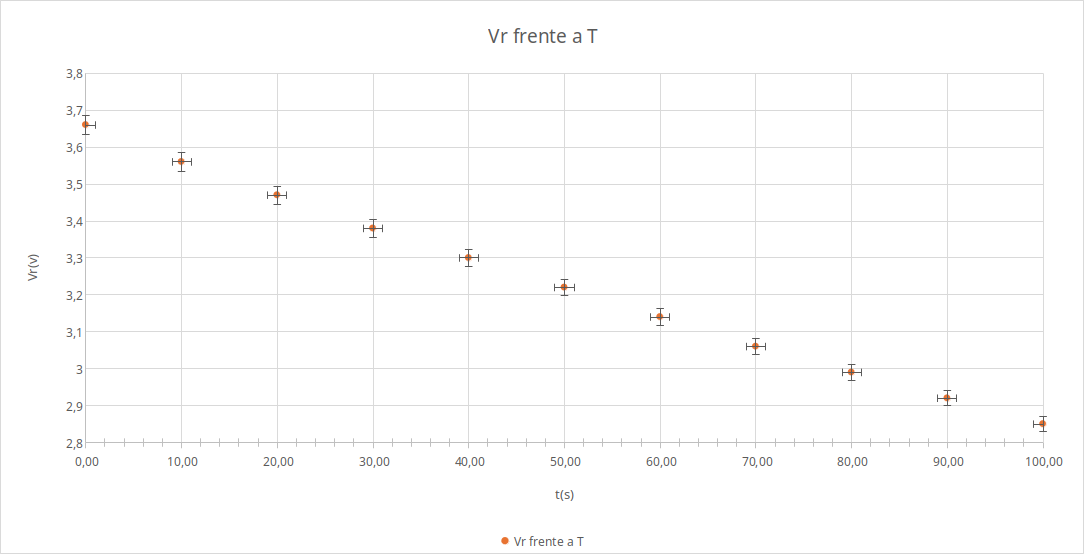
\includegraphics[width=1\linewidth]{images/graficaVr.png}
	\vspace{0.3em}
	\small{Representación gráfica de $V_R$ frente a t(s)}
 \end{figure}
\begin{figure}[H]
	\centering
	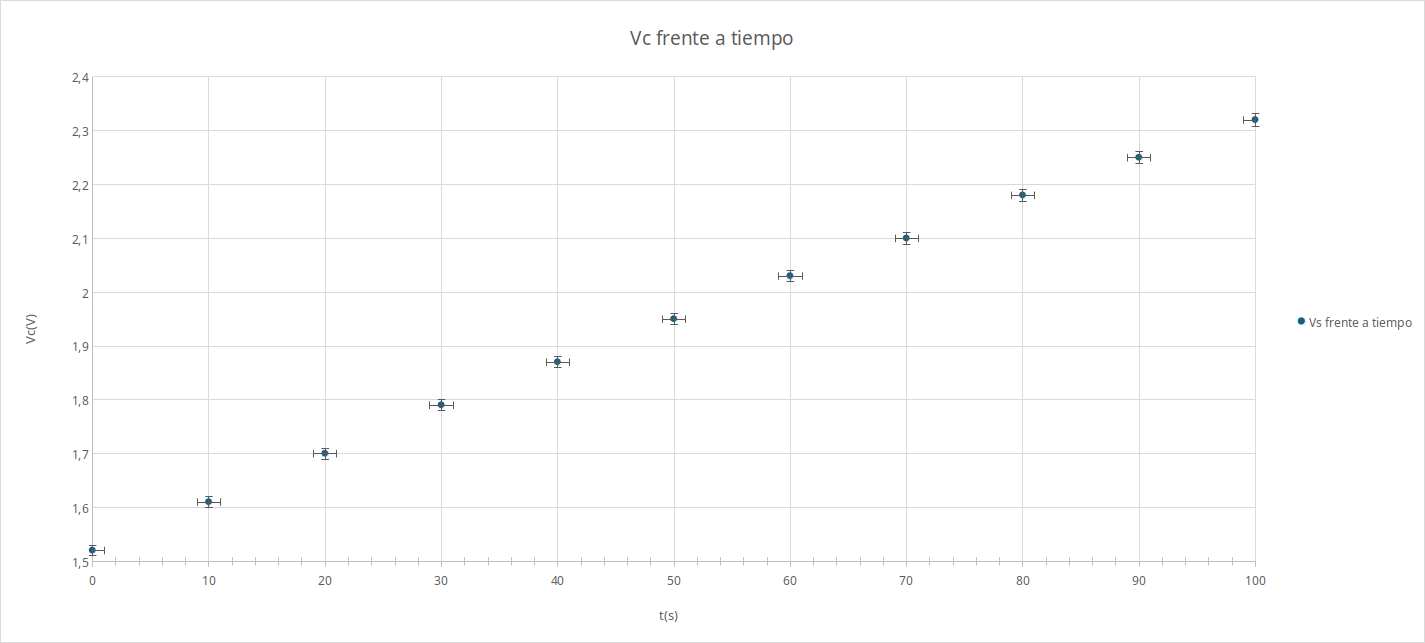
\includegraphics[width=1\linewidth]{images/graficaVc.png}
	\vspace{0.3em}
\small{Representación gráfica de $V_C$ frente a t(s)}
\end{figure}
\noindent
La expresión matemática del voltaje en la resistencia durante la descarga de un condensador en un circuito RC es una función exponencial decreciente de la forma:
\[
V_R(t) = V_0 e^{-\frac{t}{RC}},
\]
Esta ecuación describe un comportamiento característico en el que el voltaje disminuye rápidamente al inicio y se va atenuando con el tiempo, acercándose asintóticamente a cero. Por esta razón, la representación gráfica de \( V_R \) frente al tiempo muestra una curva descendente suave, coherente con el proceso de descarga exponencial típico en circuitos eléctricos de primer orden.

\vspace{2em}
\noindent
La ecuación que describe el voltaje en el condensador durante el proceso de carga en un circuito RC es:
\[
V_C(t) = V_0 \left(1 - e^{-\frac{t}{RC}}\right),
\]
Esta expresión corresponde a una función exponencial creciente, lo cual significa que el voltaje en el condensador aumenta rápidamente al inicio del proceso de carga y se va estabilizando conforme se aproxima asintóticamente a \( V_0 \). Al representar \( V_C \) frente al tiempo, se obtiene una curva ascendente suave que refleja cómo el condensador acumula carga progresivamente hasta alcanzar su valor máximo. Este comportamiento es característico de los sistemas de primer orden en respuesta a un escalón de voltaje.



\section{Q(t)}
La medida de capacitancia del condensador usado en el circuito eléctrico de carga y descarga es de:
\[
47 \eta F = 47\times10^{-6} F
\]
Ademas la capacitancia del condensador la podemos relacionar mediante la siguiente formula:
\[
C= \frac{Q}{V_c} \longrightarrow  Q (t) = C \cdot V
\]
Sustituyendo:
\[
Q(t) = 47\times10^{-6} \cdot V_c
\]
Tenemos $Q(t)$ expresado en función de $C$ y $V_c$, es decir $Q(C, V_c)$.
\vspace{1em}\\
Procedemos a calcular los errores mediante la formula genérica de propagaciones de errores, expresada matemáticamente como:
\[
\varepsilon_A = \left| \frac{\partial A}{\partial x} \right| \varepsilon_x + \left| \frac{\partial A}{\partial y} \right| \varepsilon_y
\]
En este caso concreto sustituimos y se queda:
\[
\varepsilon_Q = \left| \frac{\partial Q}{\partial C} \right| \varepsilon_C + \left| \frac{\partial Q}{\partial V_c} \right| \varepsilon_{V_c}
\]
Calculando:
\[
\left| \frac{\partial Q}{\partial C} \right| = V_c
\] 
\[
\left| \frac{\partial Q}{\partial V_c} \right| = C
\]
La expresión de propagación de errores se queda en:
\[
\varepsilon_Q = V_c \cdot \varepsilon_c + C \cdot \varepsilon_{V_c}
\]
\vspace{1em}
Ahora para poder calcular $Q(t)$ solo nos harán falta las siguientes dos expresiones:
\[
Q_i = C \cdot V_{0_i}
\]
\[
\varepsilon_{Q_i} = V_{0i} \cdot \varepsilon_C + C \cdot \varepsilon_{V_{0i}}
\]
Mediante los cálculos correspondientes con esas formulas y los datos ya mencionados llegamos a las siguientes dos tablas:
\begin{table}[H]
	\centering
	\begin{tabular}{|c|c|}
		\hline
		\textbf{$Q_i$ (C)} & \textbf{Error de $Q_i$ (C)} \\
		\hline
		\SI{7.144e-5}{}  & \SI{7.614e-6}{}  \\
		\SI{7.567e-5}{}  & \SI{8.037e-6}{}  \\
		\SI{7.990e-5}{}  & \SI{8.460e-6}{}  \\
		\SI{8.413e-5}{}  & \SI{8.883e-6}{}  \\
		\SI{8.789e-5}{}  & \SI{9.259e-6}{}  \\
		\SI{9.165e-5}{}  & \SI{9.635e-6}{}  \\
		\SI{9.541e-5}{}  & \SI{1.00181e-5}{} \\
		\SI{9.870e-5}{}  & \SI{1.03635e-5}{} \\
		\SI{1.0246e-4}{} & \SI{1.07583e-5}{} \\
		\SI{1.0575e-4}{} & \SI{1.11038e-5}{} \\
		\SI{1.0904e-4}{} & \SI{1.14492e-5}{} \\
		\hline
	\end{tabular}
\vspace{5em}
\end{table}
Representamos la evolución temporal de la carga acumulada en el condensador mediante la siguiente gráfica:

\begin{figure}[H]
	\centering
	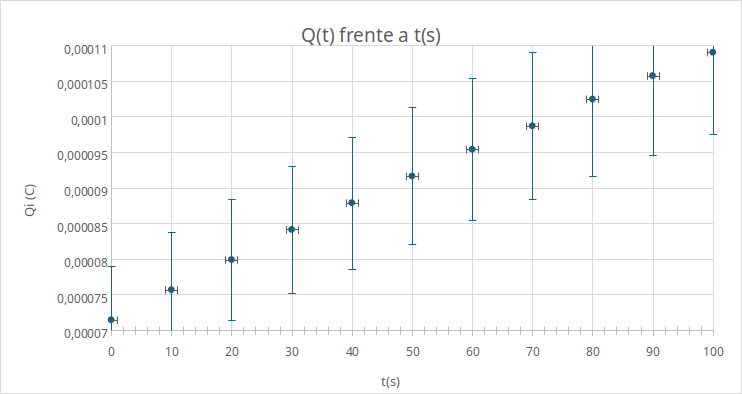
\includegraphics[width=1\linewidth]{images/graficaQt.png}
	\vspace{0.3em}
	\small{}
\end{figure}

De esta gráfica podemos empezar a sacar las primeras conclusiones. A partir de la gráfica, se observa que la carga $Q(t)$ acumulada en el condensador aumenta de forma progresiva con el tiempo, lo cual es coherente con el comportamiento esperado de un proceso de carga en un circuito RC.
Aunque no se tiene una curva ajustada explícitamente, la tendencia es claramente creciente y posiblemente lineal o exponencial en esta región inicial, como predicen las ecuaciones clásicas de carga en condensadores.

\vspace{10em}


La carga máxima que se acumula en el condensador tiene una expresión matemática de la forma:
\[
Q_{max} = V_0 \cdot C
\]
$V_0$ representa el voltaje que se le ha aplicado al circuito. Se puede calcular de una manera simple mediante la siguiente formula:
\[
V_o = \frac{V_{R_i}+V_{C_i}}{n} = \frac{V_{R_i}+V_{C_i}}{11}
\]
Por lo que con $V_R$ y $V_C$ y la formula anteriormente mencionada podemos calcular de forma simple el valor de $V_o$.
\[
V_o = 5.170 V
\]
Para calcular el error de $V_o (\varepsilon_{V_0})$ usamos la formula de la Cuasivariancia, matemáticamente:
\[
s^2 = \frac{1}{n - 1} \sum_{i=1}^{n} (x_i - \bar{x})^2
\]
que aplicada sobre $V_o$ queda la siguiente expresión:
\[
s_{V_0}^2 = \frac{1}{n - 1} \sum_{i=1}^{n} \left( V_{0i} - \overline{V_0} \right)^2
\]
esto queda:
\[
s_{V_0}^2 = 0.004 V^2
\]
Por lo que $V_0$ lo podemos expresar de la siguiente manera
\[
V_0 = (5.170 \pm 0.004) V
\]
\vspace{2em}
La carga maxima $Q_{max}$ que queriamos calcular desde el primer momento, medinate la ecuación:
\[
Q_{max} = V_0 \cdot C
\]
Ya tenemos los valores necesarios para sustituir.
\[
Q_{max} = 5.170 V \cdot 47\times10^{-6} F = 2.43 \times 10 ^{-4} C
\]
Ahora para hacerlo de manera correcta queda estimar las posibles franjas de error del valor $Q_{max}$. Esto lo haremos mediante la formula genérica de propagaciones de errores, expresada matemáticamente como:
\[
\varepsilon_A = \left| \frac{\partial A}{\partial x} \right| \varepsilon_x + \left| \frac{\partial A}{\partial y} \right| \varepsilon_y
\]
En este caso concreto sustituimos y se queda:
\[
\varepsilon_{Q_{\text{max}}} = \left| \frac{\partial Q_{\text{max}}}{\partial C} \right| \varepsilon_C + \left| \frac{\partial Q_{\text{max}}}{\partial V_0} \right| \varepsilon_{V_0}
\]
Calculando:
\[
\left| \frac{\partial Q_{\text{max}}}{\partial C} \right| = V_0
\] 
\[
\left| \frac{\partial Q_{\text{max}}}{\partial V_0} \right| = C
\]
La expresión de propagación de errores se queda en:
\[
\varepsilon_{Q_{\text{max}}} = V_0 \cdot \varepsilon_C + C \cdot \varepsilon_{V_0}
\]
Sustituyendo:
\[
\varepsilon_{Q_{\text{max}}} = 47 \times 10^{-6} \, \text{F} \times 0.004 \, \text{V} + 5.170 \, \text{V} \times 4.7 \times 10^{-6} \, \text{F} \approx 2.45 \times 10^{-5} \, \text{C}
\]
Por lo que llegamos a la expresión de $Q_{max}$.
\[
Q_{\text{max}} = \left(2.43 \times 10^{-4} \pm 2.45 \times 10^{-5} \right) \, \text{C}
\]

El valor obtenido para la carga máxima en el condensador es 
\( Q_{\text{max}} = (2.43 \pm 0.25) \times 10^{-4} \, \text{C} \), 
lo cual representa una incertidumbre aproximada del \( \sim 10\% \). 
Este nivel de error es coherente con la precisión de los instrumentos utilizados en el laboratorio, especialmente considerando que la tensión \( V_0 \) se ha estimado a partir de datos experimentales con cierta dispersión. 
Este resultado permite validar el comportamiento esperado del condensador, confirmando que la carga acumulada depende linealmente del voltaje aplicado y de la capacitancia, tal como predice la ley \( Q = C \cdot V \). 
La incorporación de la propagación de errores permite establecer un margen realista de confianza sobre la medida obtenida.
\section{V sobre resistencia}
En un circuito RC de carga/descarga, la caída de tensión en la resistencia \( R \) se describe (en la fase de descarga, por ejemplo) por la ecuación exponencial:

\[
V_R(t) = V_0 e^{-\frac{t}{\tau}},
\]
Esta forma exponencial hace que la representación directa de \( V_R \) frente a \( t \) no sea lineal. Para poder linearizar la gráfica y extraer los parámetros \( \tau \) y \( V_0 \) mediante un ajuste, se aplicará el logaritmo neperiano (\( \ln \)) a ambos lados de la ecuación. El resultado de esto queda:
\[
\ln(V_R(t)) = \ln\left(V_0 e^{-t/\tau}\right) = \ln(V_0) + \ln\left(e^{-t/\tau}\right).
\]

Dado que \( \ln(e^x) = x \), obtenemos:

\[
\ln(V_R(t)) = \ln(V_0) - \frac{t}{\tau}.
\]

\noindent
Se ha convertido la función exponencial en una función lineal de la variable \( t \).

\vspace{2em}
\noindent
La ecuación obtenida al aplicar el logaritmo natural a la expresión exponencial de \( V_R(t) \) se corresponde con una recta de la forma \( y = mx + b \). Esta se considera la recta teórica del modelo, y permite representar los datos de forma lineal. Su pendiente está relacionada con la constante de tiempo del circuito \( \tau \), y su ordenada en el origen con el valor inicial de tensión \( V_0 \). Al ajustar experimentalmente una recta a los datos transformados, se puede comparar con este modelo teórico y evaluar la validez del comportamiento exponencial del sistema.

\vspace{2em}
Por lo tanto una vez obtenida \( V_R(t) \) como una recta de la forma \( y = mx + b \), ya podemos renombrar las variables.

\[
Z \equiv \ln(V_R(t)).
\]

Entonces, la ecuación anterior queda reescrita como:

\[
Z = \ln(V_0) - \frac{t}{\tau}.
\]

Es decir, si representamos \( Z = \ln(V_R) \) en el eje vertical y \( t \) en el eje horizontal, obtenemos una recta de la forma:

\[
Z = n + mt, \quad \Longrightarrow \quad n = \ln(V_0), \quad m = -\frac{1}{\tau}.
\]

Esta linealización nos permite ajustar experimentalmente una recta a los datos transformados \( \{t_i, \ln(V_{R_i})\} \) y, a partir de ese ajuste, estimar de forma directa el valor de la constante de tiempo \( \tau \) a partir de la pendiente \( m \), así como verificar el valor de \( \ln(V_0) \) a partir de la ordenada en el origen \( n \).

\vspace{0.3cm}

Por tanto, una vez reescrita la expresión de \( \ln(V_R(t)) \) en forma de recta, se justifica el cambio de variables realizado y se habilita el tratamiento lineal de los datos experimentales, facilitando su análisis gráfico y la obtención de parámetros característicos del circuito RC.

\vspace{2em}
En este paso, se pasa de la teoría a la práctica. Ahora que hemos linealizado la ecuación, necesitamos obtener y representar los valores experimentales para extraer los parámetros \( \tau \) y \( V_0 \).

\vspace{2em}
Dados los valores de $V_R$ que ya conocemos que son:

\begin{center}
	
	\begin{table}[H]
		\centering
		\begin{tabular}{|c|c|}
			\hline
			\textbf{Índice} & \textbf{Voltaje en la resistencia $V_R$ [V]} \\
			\hline
			1  & 3.66 \\
			2  & 3.56 \\
			3  & 3.47 \\
			4  & 3.38 \\
			5  & 3.30 \\
			6  & 3.22 \\
			7  & 3.14 \\
			8  & 3.06 \\
			9  & 2.99 \\
			10 & 2.92 \\
			11 & 2.85 \\
			\hline
		\end{tabular}

	\end{table}
	
\end{center}



Ahora para cada valor de \( V_R(t_i) \), se aplica el logaritmo neperiano, con la expresión:

\[
Z_i = \ln(V_R(t_i)).
\]

Estos valores \( Z_i \) son los que, según la teoría, deberían ajustarse a una recta en función de \( t_i \).

\vspace{1.5em}

Una vez aplicado los $ln$ te quedan los siguientes datos:

\begin{center}
\begin{table}[H]
	\centering
	\begin{tabular}{|c|c|}
		\hline
		\textbf{Índice} & \textbf{$\ln(V_R)$} \\
		\hline
		1  & 1.2975 \\
		2  & 1.2698 \\
		3  & 1.2442 \\
		4  & 1.2179 \\
		5  & 1.1939 \\
		6  & 1.1694 \\
		7  & 1.1442 \\
		8  & 1.1184 \\
		9  & 1.0953 \\
		10 & 1.0716 \\
		11 & 1.0473 \\
		\hline
	\end{tabular}
\end{table}
\end{center}

\vspace{2em}
Ahora necesitamos conocer el error de $\ln(V_R)$, primero debemos expresar:
\[
f = \ln(V_R)
\] para ello utilizamos la formula genérica de propagaciones de errores, expresada matemáticamente como:
\[
\varepsilon_A = \left| \frac{\partial A}{\partial x} \right| \varepsilon_x
\]
En este caso concreto sustituimos y se queda:
\[
\varepsilon_f = \left| \frac{\partial f}{\partial V_R} \right| \varepsilon_{V_R}
\]
Calculando:
\[
\left| \frac{\partial f}{\partial V_R} \right| = \frac{1}{V_R}
\] 
La expresión de propagación de errores se queda en:
\[
\varepsilon_Q = \frac{1}{V_R} \cdot \varepsilon_{V_R}
\]
Operando, nos queda la siguiente tabla con los errores de $V_R$:
\begin{table}[H]
	\centering
	\begin{tabular}{|c|c|}
		\hline
		\textbf{Índice} & \textbf{Error de $\ln(V_R)$} \\
		\hline
		1  & 0.007 \\
		2  & 0.007 \\
		3  & 0.007 \\
		4  & 0.007 \\
		5  & 0.007 \\
		6  & 0.007 \\
		7  & 0.007 \\
		8  & 0.007 \\
		9  & 0.007 \\
		10 & 0.007 \\
		11 & 0.007 \\
		\hline
	\end{tabular}
\end{table}

Una vez conocidos los errores de $ln(V_R)$ ya podemos graficar $ln(V_R)$ frente al tiempo, de manera que queda:
 \begin{figure}[H]
 	\centering
 	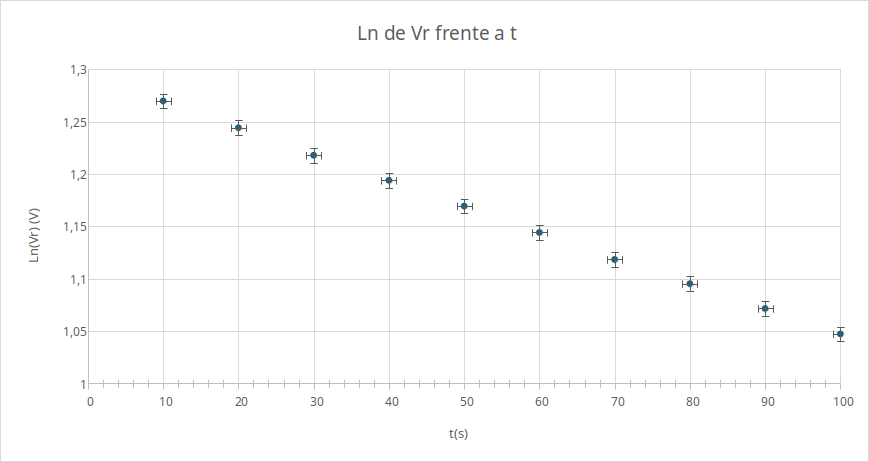
\includegraphics[width=1\linewidth]{images/graficaLnVr.png}

 \end{figure}
 
\vspace{4em}

Para sacar los datos de $Z$, que recordamos que es:
\[
Z = \ln(V_0) - \frac{t}{\tau}.
\]
Lo hacemos mediante el uso de la regresión lineal, que hace uso de la siguiente expresión:
\[
Z = mt + n
\]

\[
m = \frac{n \sum t_i Z_i - \sum t_i \sum Z_i}{n \sum t_i^2 - \left(\sum t_i\right)^2}
\]

\[
n = \frac{\sum Z_i - m \sum t_i}{n}
\]
Operamos y nos queda:
\[
m = \text{(pendiente)} = -\frac{1}{\tau} \approx -0.002489
\]
\[
n = \text{(ordenada)} = \ln(V_0) \approx 1.2944
\]
Con sus errores correspondientes:
\[
\varepsilon_m \approx 1.51672 \times 10^{-5}
\]
\[
\varepsilon_n \approx 8.97303 \times 10^{-4}
\]
Finalmente, se concluye en esto:
\[
\ln(V_R) = (1.2944 \pm 0.0009) + (-0.00249 \pm 0.00002)\, t
\]
Con estos datos podemos, tratar de hacer una aproximación de $\tau$ y $V_0$.
\[
m = -\frac{1}{\tau} \longrightarrow \tau = -\frac{1}{-m} \approx \frac{1}{-0.002489} \approx 401.6 s
\]
\[
n = \ln(V_0) \longrightarrow V_0 \approx e^{n} \approx e^{1.2944} \approx 3.65 V
\]
Ademas la regresión lineal da un valor de:
\[
R^2 \approx 0.9997
\]
Esto quiere decir que la recta se ajusta muy bien a los datos, lo que confirma el modelo experimental

\vspace{3em}


Para calcular el error asociado a \( \tau \), denotado como \( \varepsilon_\tau \), se aplica la fórmula de propagación de errores a la función \( \tau(m) = -1/m \), considerando su dependencia exclusiva respecto a \( m \). El error absoluto se expresa como:

\[
\varepsilon_\tau = \left| \frac{d\tau}{dm} \right| \cdot \varepsilon_m = \left| \frac{1}{m^2} \right| \cdot \varepsilon_m,
\]
entonces:
\vspace{0.3cm}


\begin{align*}
	m &= -0.00249, \quad \varepsilon_m = 0.00002, \\
	\varepsilon_\tau &= \frac{\varepsilon_m}{m^2} = \frac{0.00002}{(-0.00249)^2} \approx 3.2 \text{ s}.
\end{align*}

Por tanto, la constante de tiempo con su error absoluto puede expresarse como:
\[
\tau = (401.6 \pm 3.2) \, \text{s}.
\]
Por otra parte, considerando que la ordenada en el origen del ajuste lineal es \( n = \ln(V_0) \), para calcular el error asociado a \( V_0 \), denotado como \( \varepsilon_{V_0} \), se aplica nuevamente la fórmula de propagación de errores mediante derivación, considerando únicamente la dependencia respecto a \( n \). El resultado es:

\[
\varepsilon_{V_0} = \left| \frac{dV_0}{dn} \right| \cdot \varepsilon_n = \left| e^n \right| \cdot \varepsilon_n = V_0 \cdot \varepsilon_n,
\]


\vspace{0.3cm}



\begin{align*}
	n &= 1.2944, \quad \varepsilon_n = 0.000897, \\
	\varepsilon_{V_0} &= 3.65 \cdot 0.000897 \approx 0.0033 \, \text{V}.
\end{align*}

Por tanto, se puede expresar el valor de \( V_0 \) con su error como:

\[
V_0 = (3.65 \pm 0.003) \, \text{V}.
\]
Ahora vamos a comparar $\tau$, para ello vamos a aplicar la formula del error relativo porcentual, donde vamos a comparar $\tau_{exp}$ y $\tau_{teo}$
\vspace{2em}
El valor de $\tau_{exp}$ ya lo sabemos y es de:
\[
\tau = (401.6 \pm 3.2) \, \text{s}.
\]
Ahora $\tau_{teo}$, tiene la formula de:
\[
\tau_{exp} = R \cdot C
\] 


Sabemos los datos de:
\[
C = 47\times10^{-6} F
\]
\[
R = 7.07\times10^{6}\varOmega
\]
Por lo que:
\[
\tau_{exp} = R \cdot C = 7.07\times10^{6}\varOmega \cdot 47\times10^{-6} F \approx 332.29
\] 
Ahora mediante la ecuación del error relativo porcentual, que se expresa como:
\[
\text{Error relativo (\%)} = \left| \frac{\tau_{\text{exp}} - \tau_{\text{teo}}}{\tau_{\text{teo}}} \right| \cdot 100
\]
Con los valores:
\[
\text{Error relativo (\%)} = \left| \frac{401.6 - 334.64}{334.64} \right| \cdot 100 \approx 20.1\%
\]
Este resultado indica que el valor experimental se encuentra razonablemente próximo al valor teórico, con una diferencia del orden del $20.1$





\end{document}
